\section{Boxplot: Summarizing Data at a Glance}

Imagine you’re trying to quickly understand how students performed in a test—not just where most scores lie, but also how consistent the scores are and whether any students performed exceptionally well or poorly. A boxplot (also called a box-and-whisker plot) helps us do exactly that.

\subsection*{Key Concepts: Let’s Explore!}

Boxplots are used for numerical data. They show five important numbers that summarize the data:
\begin{itemize}
  \item \textbf{Minimum}: The lowest value in the dataset (excluding extreme outliers).
  \item \textbf{First Quartile (Q1)}: The value below which 25\% of the data falls.
  \item \textbf{Median (Q2)}: The middle value that divides the data into two equal halves.
  \item \textbf{Third Quartile (Q3)}: The value below which 75\% of the data falls.
  \item \textbf{Maximum}: The highest value in the dataset (excluding extreme outliers).
\end{itemize}

\textit{Activity: Can you identify these five values in a small dataset of test scores? Try with: 42, 55, 60, 65, 70, 75, 90}

\paragraph{The Box and the Whiskers}

The box spans from the first quartile (Q1) to the third quartile (Q3). This shows where the middle 50\% of the data lies. It helps us understand the data’s “interquartile range” or IQR.

A line inside the box marks the median.

The whiskers extend from the box to the minimum and maximum values that are not considered outliers.

Any points that lie far outside the whiskers are called outliers and are usually plotted as individual dots or stars.

\subsection*{Why Use Boxplots?}

Boxplots help us see:
\begin{itemize}
  \item \textbf{Skewness}: If the median is not centered in the box or if one whisker is much longer, the data may be skewed.
  \item \textbf{Spread}: A longer box or whiskers mean more variability in the data.
  \item \textbf{Outliers}: Easily spot values that don’t fit the general pattern.
  \item \textbf{Comparison}: Boxplots are great for comparing multiple datasets side by side.
\end{itemize}

\paragraph{Visual Summary: What You Learn at a Glance}

\begin{itemize}
  \item A centered median suggests a symmetric distribution.
  \item A longer upper whisker might suggest a few students scored exceptionally high.
  \item Outliers could represent unusual performances or data entry errors.
\end{itemize}

\subsection*{Example: Let’s Visualize Climate Data}

We can apply a boxplot to climate data to understand temperature variations over the years. For instance, let’s consider the average summer temperature across several years. A boxplot can quickly show:
\begin{itemize}
  \item Whether the temperatures have a consistent range.
  \item If there are any outlier years with unusually hot or cold summers.
  \item Whether the trend has become skewed (perhaps due to climate change).
\end{itemize}

\subsection*{Try it in R!}

\paragraph{Wind Speed Analysis by Altitude}

Wind speed is a crucial component of climate data and can vary significantly with altitude. In this task, we explore how wind speed differs between two common measurement heights: 10 meters and 50 meters above ground level.

Understanding wind speed variability at different altitudes is important for:
\begin{itemize}
  \item Weather forecasting: Accurate wind speed data improves storm tracking and model predictions.
  \item Agricultural planning: Wind affects crop pollination, irrigation patterns, and soil erosion.
  \item Environmental studies: Wind disperses pollutants and influences temperature and humidity distribution.
\end{itemize}

\paragraph{Step 1: Summary Statistics in R}

First, we calculate summary statistics for wind speed at both altitudes using the \texttt{dplyr} package in R:

\begin{verbatim}
summary <- climate_data %>%
  summarise(
    mean_10m = mean(WindSpeed_10m),
    sd_10m = sd(WindSpeed_10m),
    median_10m = median(WindSpeed_10m),
    mean_50m = mean(WindSpeed_50m),
    sd_50m = sd(WindSpeed_50m),
    median_50m = median(WindSpeed_50m)
  )
print(summary)
\end{verbatim}

% Fihgure here -------------------------
\begin{figure}[h]
\centering
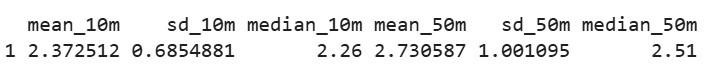
\includegraphics[width=0.6\textwidth]{figures/summ_stats.jpg}
\caption{Summary Statistics}
\end{figure}

This code computes:
\begin{itemize}
  \item Mean: The average wind speed at each height.
  \item Standard deviation (SD): How much the wind speed varies from the mean.
  \item Median: The middle value in the dataset.
\end{itemize}
These measures help us compare central tendency and variability between the two heights.

\paragraph{Step 2: Visual Comparison using Boxplot}

We now visualize the wind speeds using a boxplot:

\begin{verbatim}
boxplot(
  climate_data$WindSpeed_10m, climate_data$MaxWindSpeed_50m,
  names = c("WindSpeed_10m","WindSpeed_50m"),
  main = "Windspeed Comparison",
  xlab = "Windspeed (m/s)",
  col = c("green", "orange")
)
\end{verbatim}

% Figure ------------------------------
\begin{figure}[h]
\centering
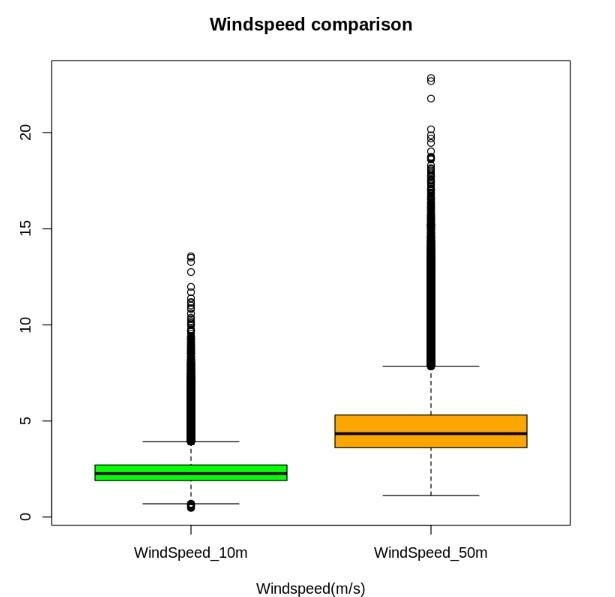
\includegraphics[width=0.5\textwidth]{figures/windspeed.jpg}
\caption{Windspeed Comparison at 10m and 50m}
\end{figure}

This boxplot compares the distribution of wind speed at 10m and 50m heights. Here’s what we observe:
\begin{itemize}
  \item \textbf{Median Line}: Indicates the central value of wind speed for each altitude.
  \item \textbf{Box Size}: Represents the interquartile range (spread of the middle 50\% of values).
  \item \textbf{Whiskers and Outliers}: Show the overall range and any extreme values.
\end{itemize}

\textbf{Discussion} \\

Typically, wind speed increases with altitude due to reduced friction with the Earth’s surface. Therefore, we expect the boxplot for 50m to have:
\begin{itemize}
  \item A higher median compared to 10m.
  \item Possibly greater variability, depending on terrain and weather conditions.
\end{itemize}

\textit{Activity: Can you interpret the difference in medians and spreads between the two boxplots? What might this tell us about wind behavior in the area?}

This analysis demonstrates how simple statistics and visualizations can uncover meaningful patterns in climate data, helping us make more informed decisions in environmental monitoring and planning.

\subsection*{Outliers and Their Significance in Climate Data}

Outliers are data points that significantly deviate from the general pattern of the dataset. In the context of climate analysis, outliers may represent unusual or extreme weather events—such as unexpected temperature spikes, intense rainfall, or strong windstorms. These anomalies are critical for several reasons:
\begin{itemize}
  \item \textbf{Insights into Extreme Events}: Outliers can help identify climatic extremes such as droughts, floods, or heatwaves. Recognizing these events is vital for disaster preparedness and mitigation.
  \item \textbf{Indicators of Data Quality Issues}: Outliers can sometimes indicate sensor errors or mistakes in data recording, highlighting the need for validation.
  \item \textbf{Understanding Climate Trends}: Persistent or frequent outliers might signal larger shifts in climate patterns.
  \item \textbf{Impact on Modeling}: Since outliers can skew statistical models, identifying and treating them appropriately is essential for producing reliable predictions.
\end{itemize}

\textbf{Interquartile Range (IQR) Method for Detecting Outliers}\\

The IQR is a measure of variability, defined as the difference between the third quartile (Q3) and the first quartile (Q1):
\[
\text{IQR} = Q_3 - Q_1
\]

Data points falling outside the following bounds are considered potential outliers:
\[
\text{Lower Bound} = Q_1 - 1.5 \times \text{IQR}, \quad \text{Upper Bound} = Q_3 + 1.5 \times \text{IQR}
\]

\paragraph{R Code: Identifying Outliers Based on Precipitation}

\begin{verbatim}
# Step 1: Calculate IQR and Bounds
Q1 <- quantile(filtered_hilly_data$Precip, 0.25)  # First Quartile (25%)
Q3 <- quantile(filtered_hilly_data$Precip, 0.75)  # Third Quartile (75%)
IQR <- Q3 - Q1  # Interquartile Range
lower_bound <- Q1 - 1.5 * IQR  # Lower bound
upper_bound <- Q3 + 1.5 * IQR  # Upper bound

# Step 2: Identify Outliers
outliers <- filtered_hilly_data
[filtered_hilly_data$Precip <
 lower_bound | filtered_hilly_data$Precip > upper_bound, ]
non_outliers <- filtered_hilly_data
[filtered_hilly_data$Precip >= 
lower_bound & filtered_hilly_data$Precip <= upper_bound, ]
\end{verbatim}

\textbf{Summary Statistics with and without Outliers} \\

Summary statistics are numerical values that describe key features of a dataset. These include measures of central tendency and variability, and are essential for understanding the general behavior of climate data.

\begin{verbatim}
cat("Original Dataset Summary:\n")
summary(filtered_hilly_data$Precip)

cat("\nDataset Without Outliers:\n")
summary(non_outliers$Precip)

cat("\nOutliers Only:\n")
summary(outliers$Precip)
\end{verbatim}

% Figure --------------------------------
\begin{figure}[h]
\centering
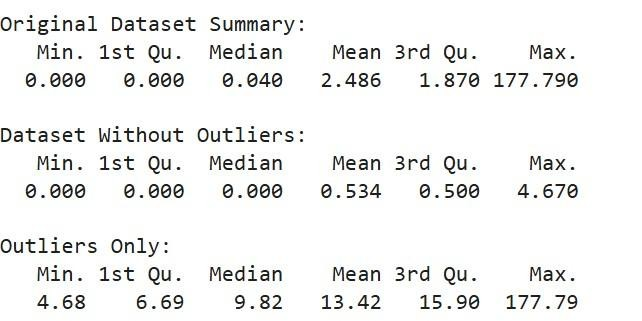
\includegraphics[width=0.6\textwidth]{figures/summary_stats.jpg}
\caption{Summary Statistics}
\end{figure}

\subsection*{Visualizing Outliers with Boxplots} 

\subsubsection*{Boxplot including outliers:}

\begin{verbatim}
ggplot(filtered_hilly_data, aes(x = Month_Label, y = Precip)) +
  geom_boxplot(outliers.colour = "red") +
  theme_minimal() +
  labs(
    title = "Precipitation Variation by Seasons", 
    x = "Month", 
    y = "Precipitation"
    )
\end{verbatim}

\subsubsection*{Boxplot without outliers:}

\begin{verbatim}
ggplot(non_outliers, aes(x = Month_Label, y = Precip)) +
  geom_boxplot() +
  theme_minimal() +
  labs(
    title = "Precipitation Variation by Seasons",
    x = "Month",
    y = "Precipitation"
    )
\end{verbatim}

% Figure here-----------------------------
\begin{figure}[h]
\centering
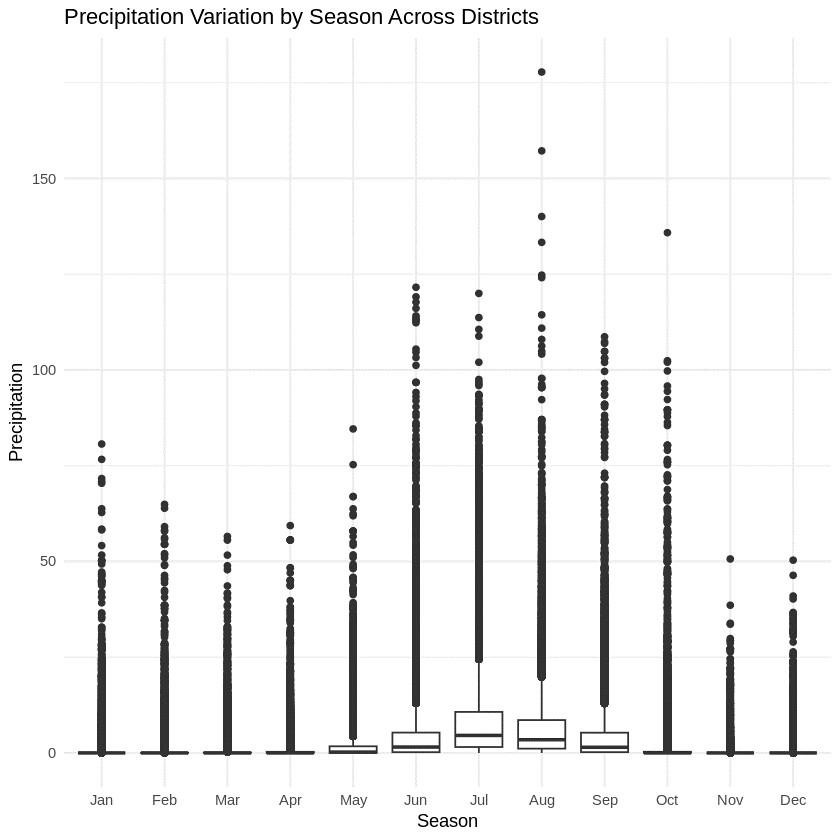
\includegraphics[width=0.5\textwidth]{figures/outliers.jpg}
\caption{Boxplot Showing Outliers}
\end{figure}

% Figure here-----------------------------
\begin{figure}[h]
\centering
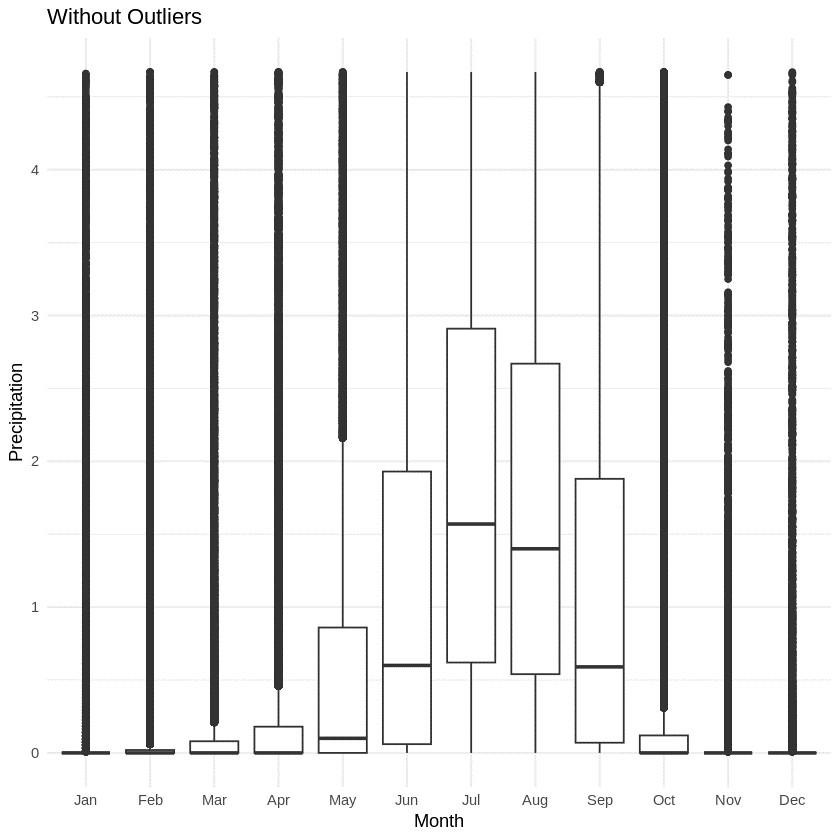
\includegraphics[width=0.5\textwidth]{figures/no_outliers.jpg}
\caption{Boxplot After Removing Outliers}
\end{figure}

\subsection*{Understanding Standard Deviation and Range}

\textbf{1. Standard Deviation}\\

Standard deviation quantifies how much the data deviates from the mean. A higher value indicates that the data points are more spread out, while a lower value suggests they are clustered around the mean.

\paragraph{Formula for Population Standard Deviation:}
\[
\sigma = \sqrt{\frac{1}{N} \sum_{i=1}^N (x_i - \mu)^2}
\]

\paragraph{Formula for Sample Standard Deviation (with Bessel’s correction):}
\[
s = \sqrt{\frac{1}{N-1} \sum_{i=1}^N (x_i - \bar{x})^2}
\]

\paragraph{Interpretation:}
\begin{itemize}
  \item Low standard deviation \(\rightarrow\) Values are close to the mean.
  \item High standard deviation \(\rightarrow\) Values are widely spread.
\end{itemize}

\paragraph{2. Range}

The range is the difference between the maximum and minimum values in the dataset:
\[
\text{Range} = \text{Maximum} - \text{Minimum}
\]

\paragraph{Interpretation:}
\begin{itemize}
  \item Small range \(\rightarrow\) Values are concentrated.
  \item Large range \(\rightarrow\) Values are spread out, possibly due to outliers.
\end{itemize}

\paragraph{R Code: Calculating Standard Deviation and Range}

\begin{verbatim}
cat("\nStandard Deviation with Outliers: ", 
sd(filtered_hilly_data$Precip), "\n")
cat("Standard Deviation without Outliers: ", 
sd(non_outliers$Precip), "\n")

cat("\nRange with Outliers: ", range(filtered_hilly_data$Precip), "\n")
cat("Range without Outliers: ", range(non_outliers$Precip), "\n")
\end{verbatim}

% Figure here--------------------------
\begin{figure}[h]
\centering
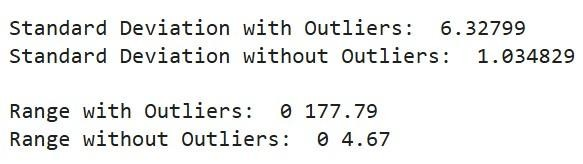
\includegraphics[width=0.6\textwidth]{figures/sd_range.jpg}
\caption{Standard Deviation and Range Calculation}
\end{figure}

\paragraph{Results Interpretation}

\begin{itemize}
  \item \textbf{Standard Deviation}:
  \begin{itemize}
    \item With outliers: 6.33
    \item Without outliers: 1.03
  \end{itemize}
  Outliers significantly increase the standard deviation, exaggerating the variability in precipitation data.
  
  \item \textbf{Range}:
  \begin{itemize}
    \item With outliers: 0 to 177.79
    \item Without outliers: 0 to 4.67
  \end{itemize}
  The range is greatly inflated by extreme values, demonstrating how outliers can distort the data distribution.
\end{itemize}

\paragraph{Points to Note}

\begin{itemize}
  \item Outliers make the data appear more variable than it actually is.
  \item Removing outliers can help clarify typical climate patterns.
  \item If the goal is to understand extreme events (like floods or heavy rain), outliers should be analyzed, not discarded.
\end{itemize}
However, if you’re trying to understand the more typical patterns in the data, removing the outliers might give you a clearer picture.

\clearpage
